\chapter{Additional Figures}
\label{app:figures}


\section{\ttZ Preselection}
Additional figures showing distribations of variables with a relaxed selection. The selection applied is similar to the full selection but lacking the requirement of 4 jets (only 2 b-tags required). 
\begin{figure}[h]
\begin{center}
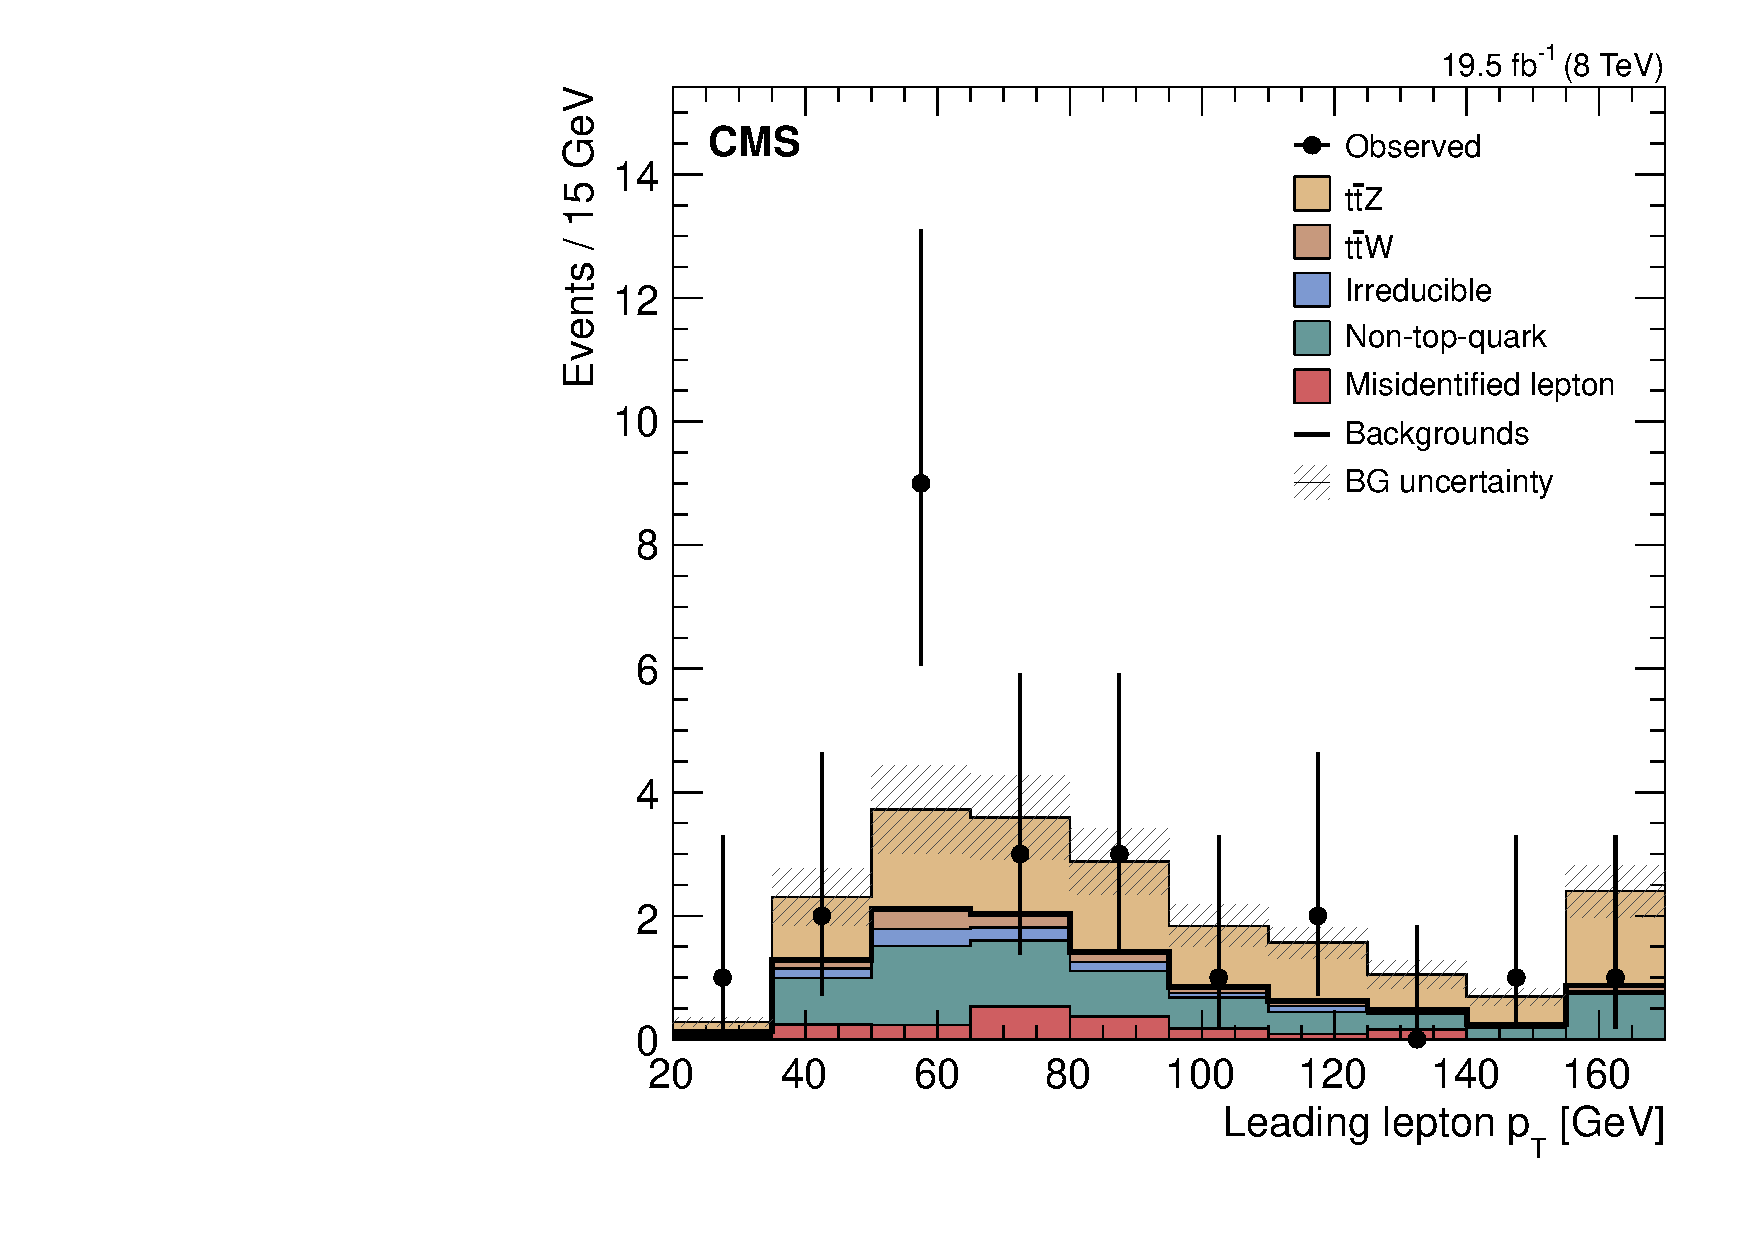
\includegraphics[width=0.48\linewidth]{Figs/Plots_PreSelections/hZLep1Pt_3L2b.pdf}
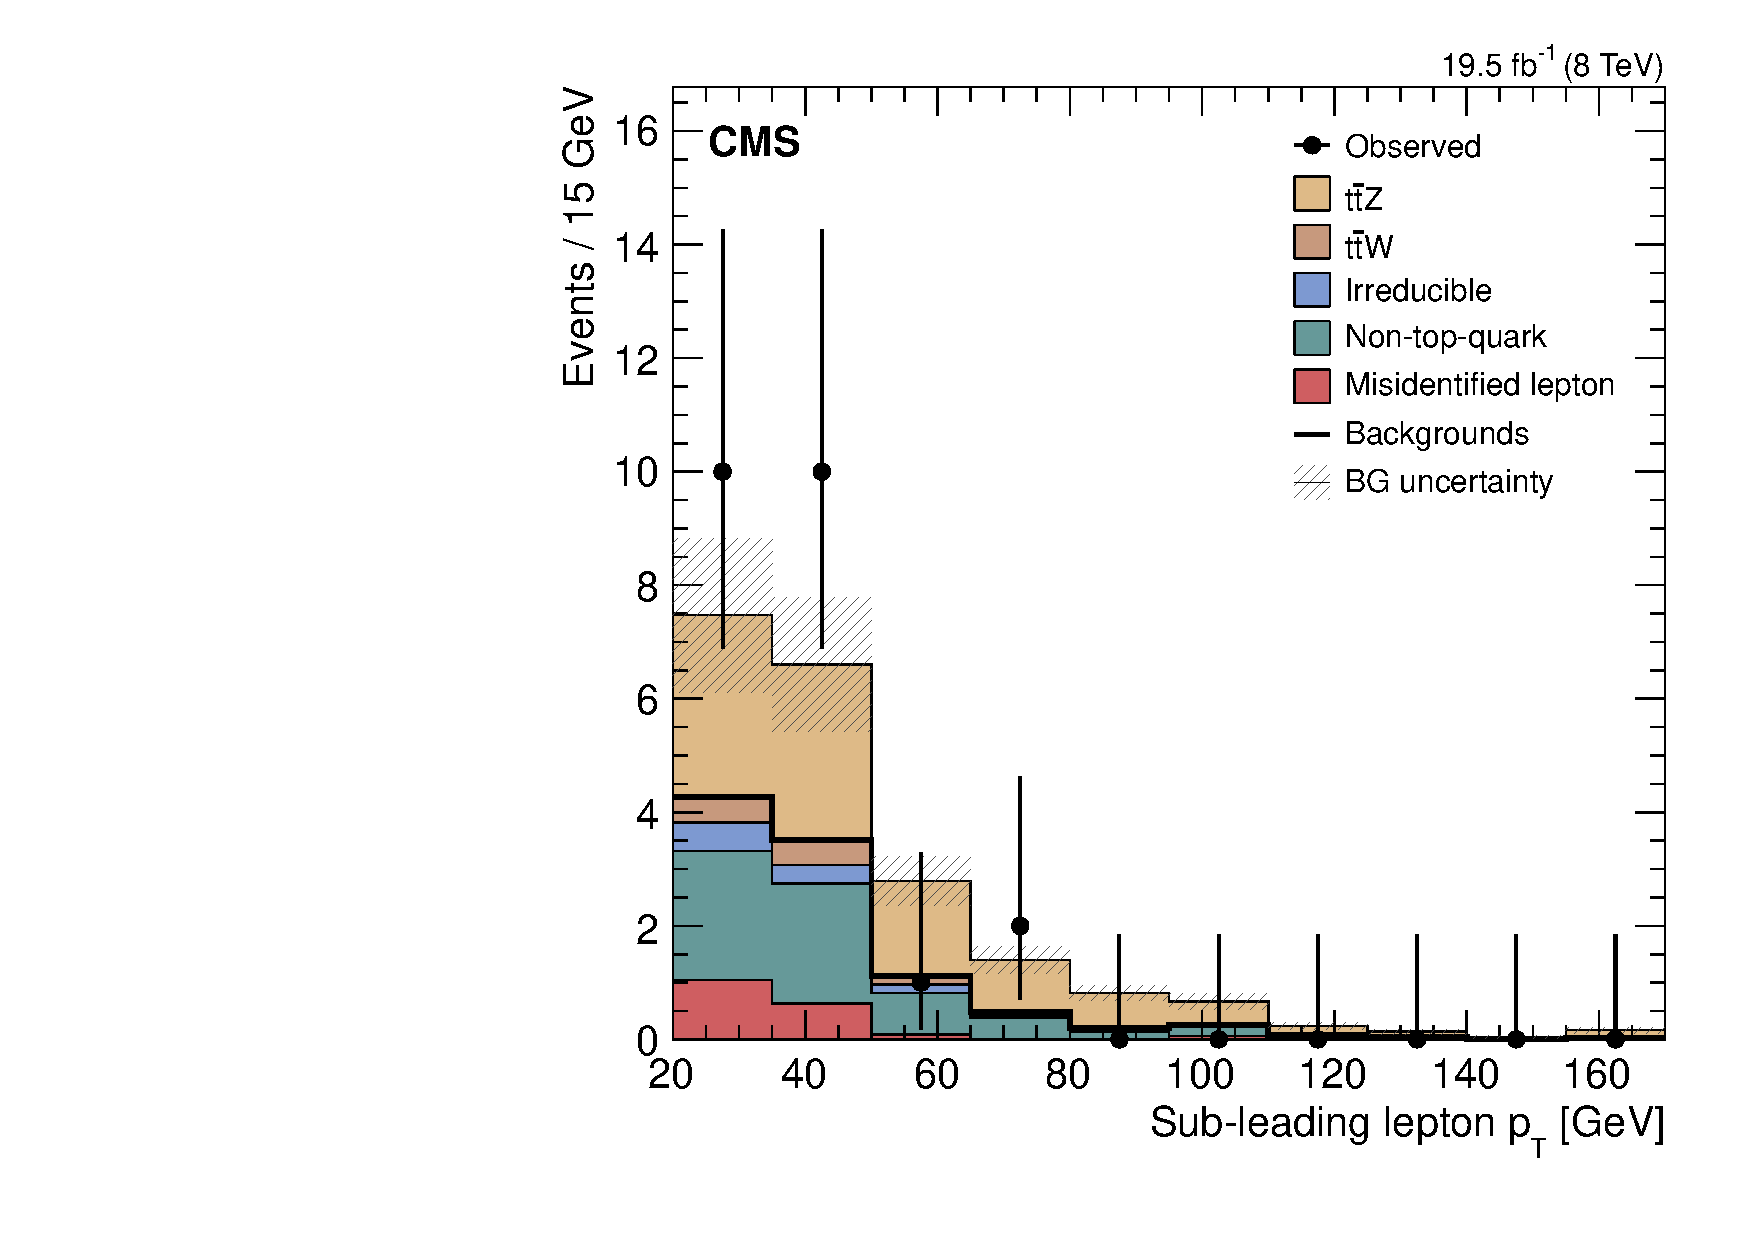
\includegraphics[width=0.48\linewidth]{Figs/Plots_PreSelections/hZLep2Pt_3L2b.pdf}
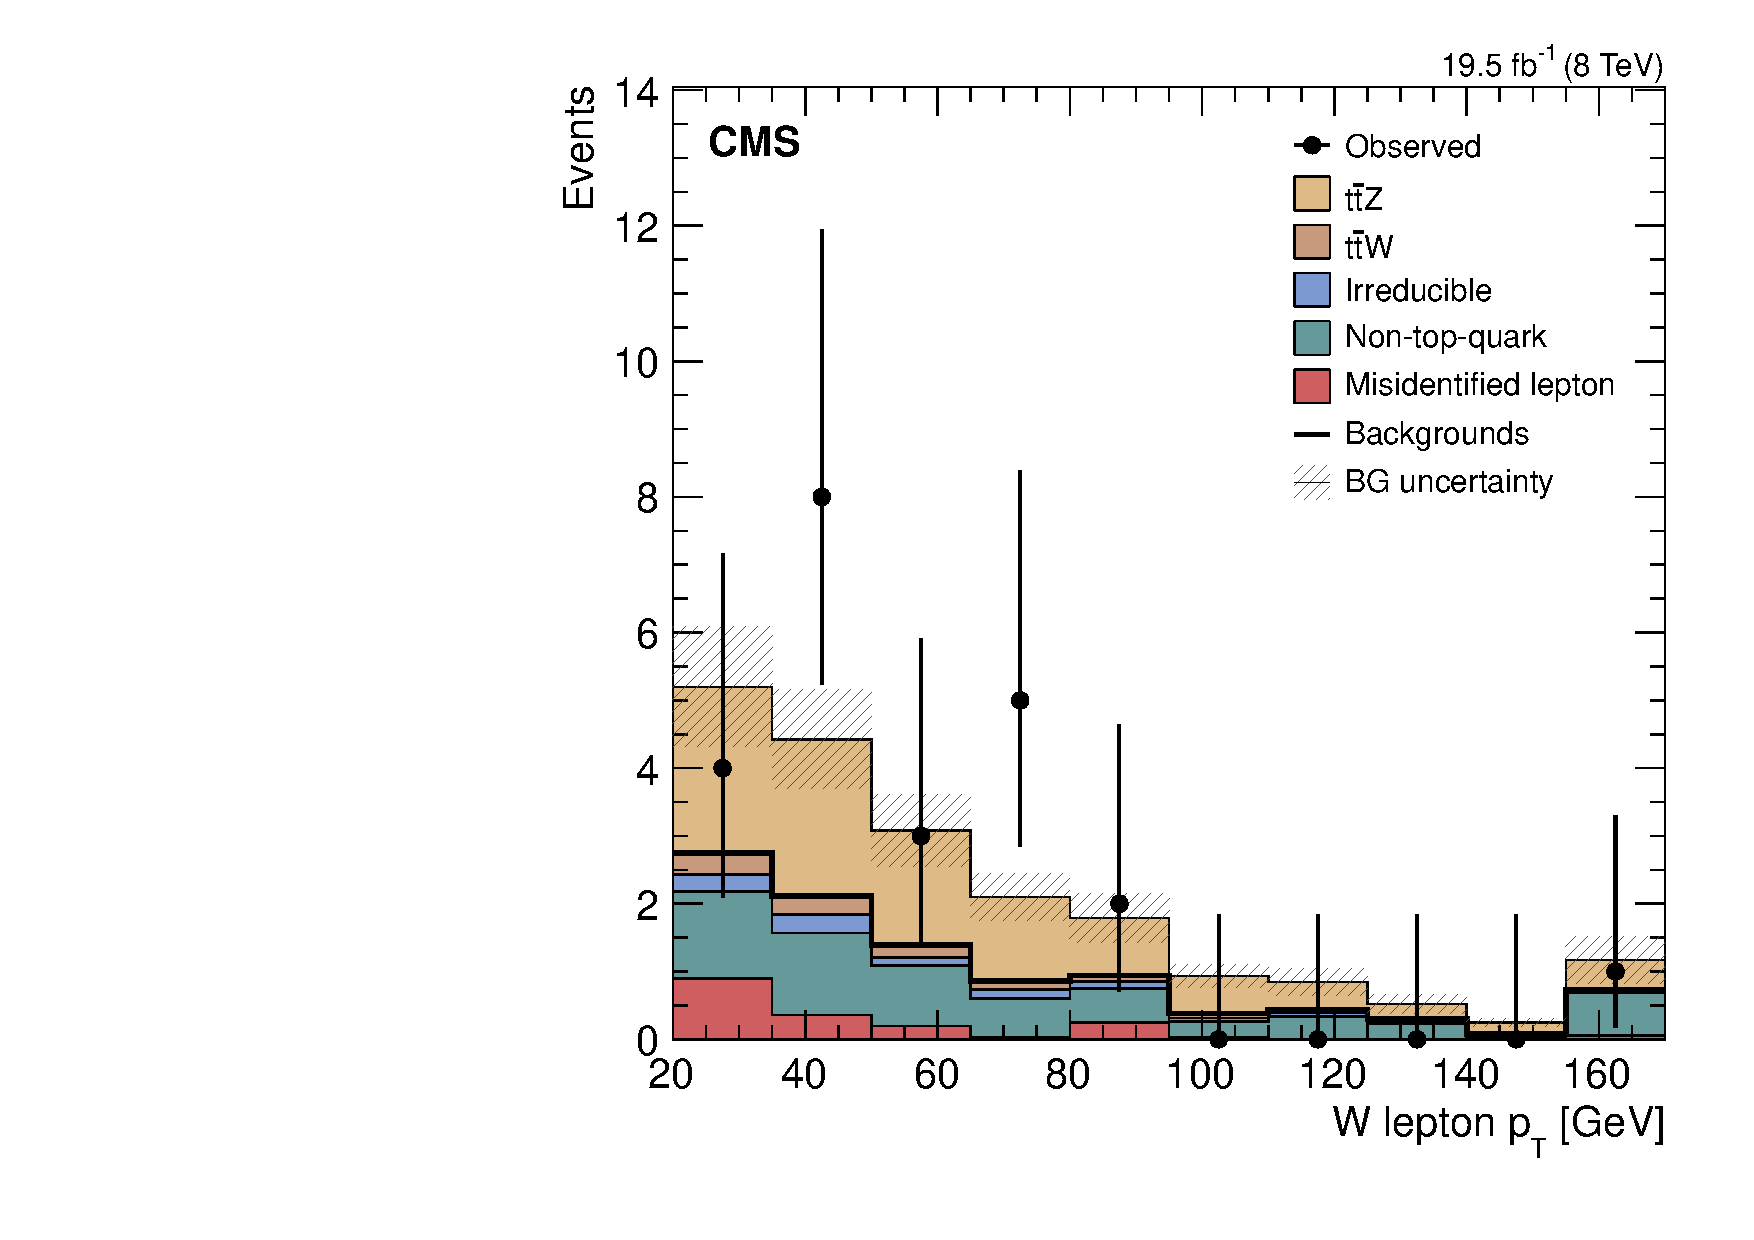
\includegraphics[width=0.48\linewidth]{Figs/Plots_PreSelections/hWLepPt_3L2b.pdf}
\caption{\label{fig:hleppt_3L2b}
\pt of the Z and W leptons after tri-lepton plus two b-tag selections. Left: Leading Pt lepton. Right: Trailing \pt lepton. Bottom: W lepton.
}
\end{center}
\end{figure}




\begin{figure}[h]
\begin{center}
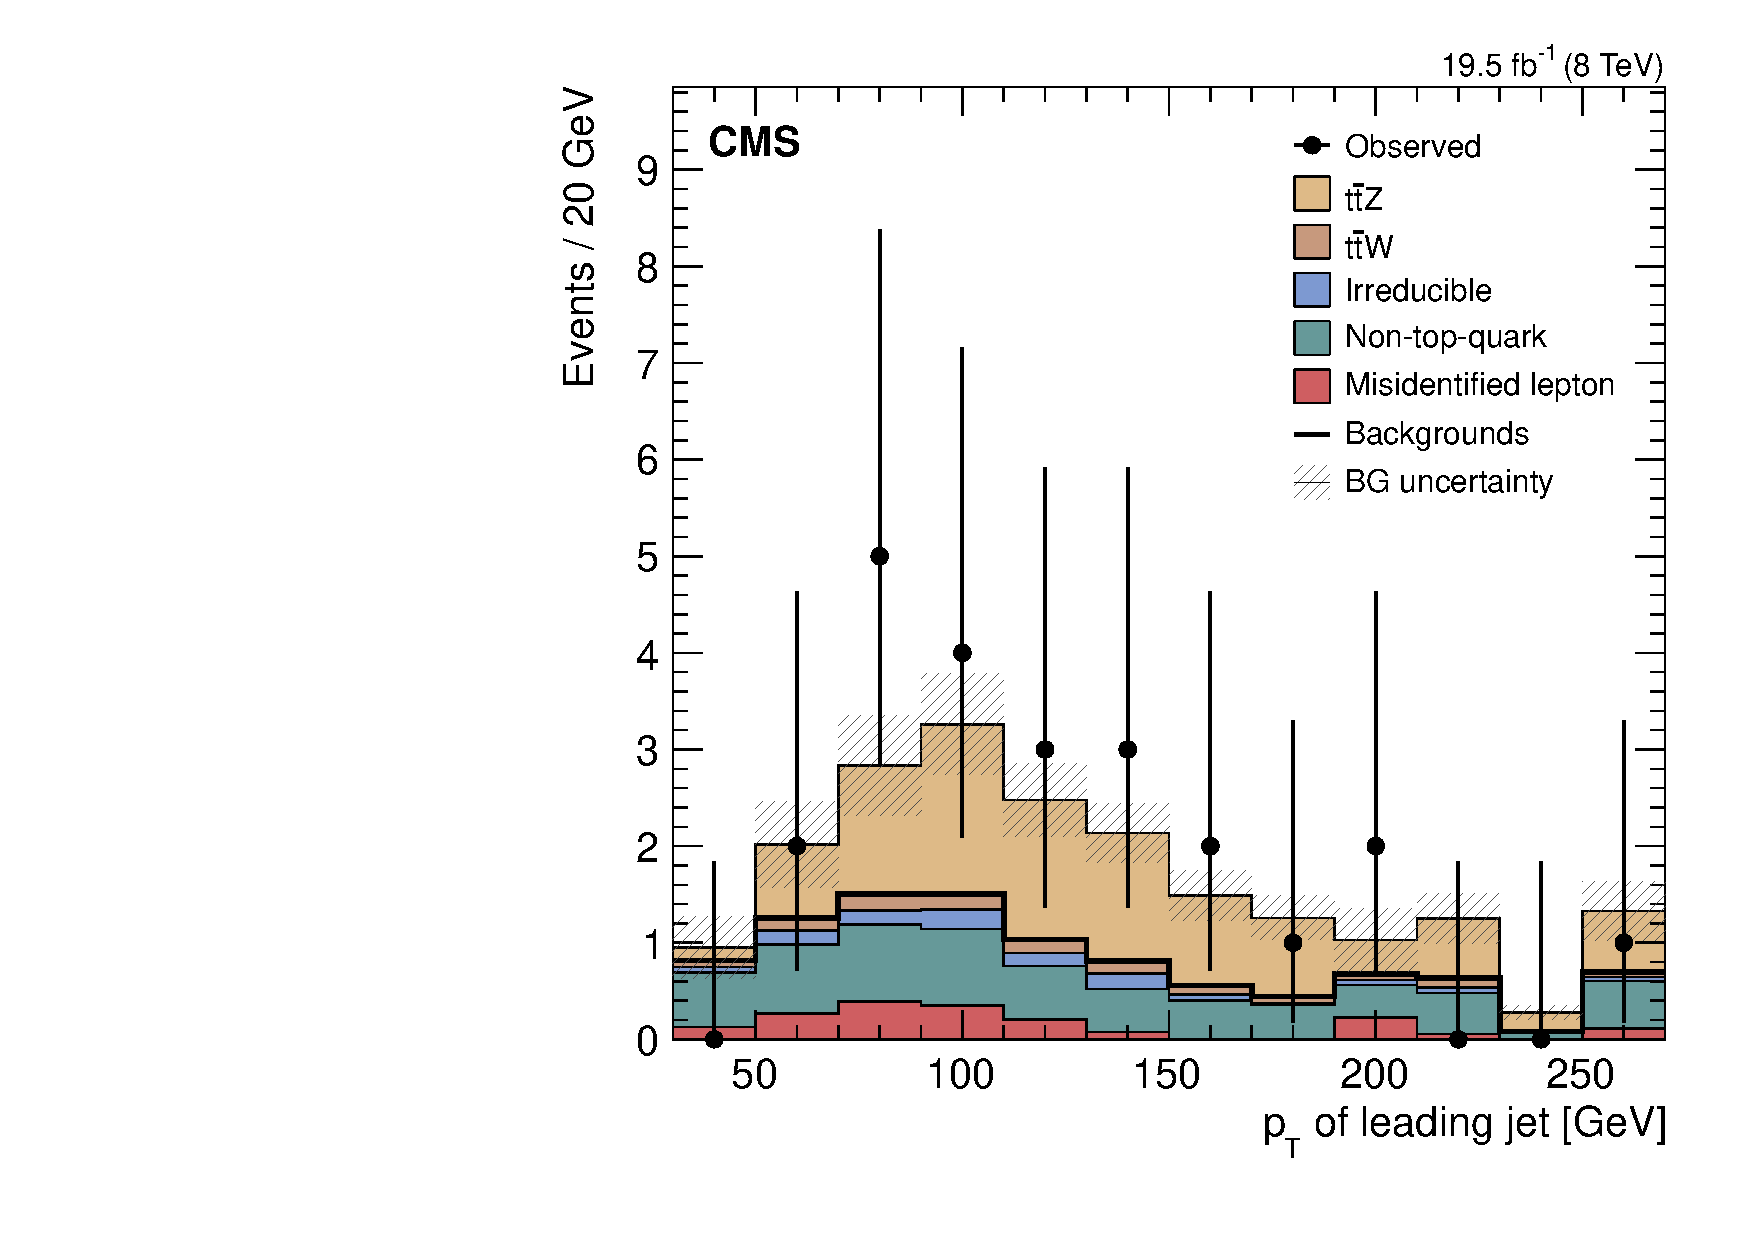
\includegraphics[width=0.48\linewidth]{Figs/Plots_PreSelections/hJ1Pt_3L2b.pdf}
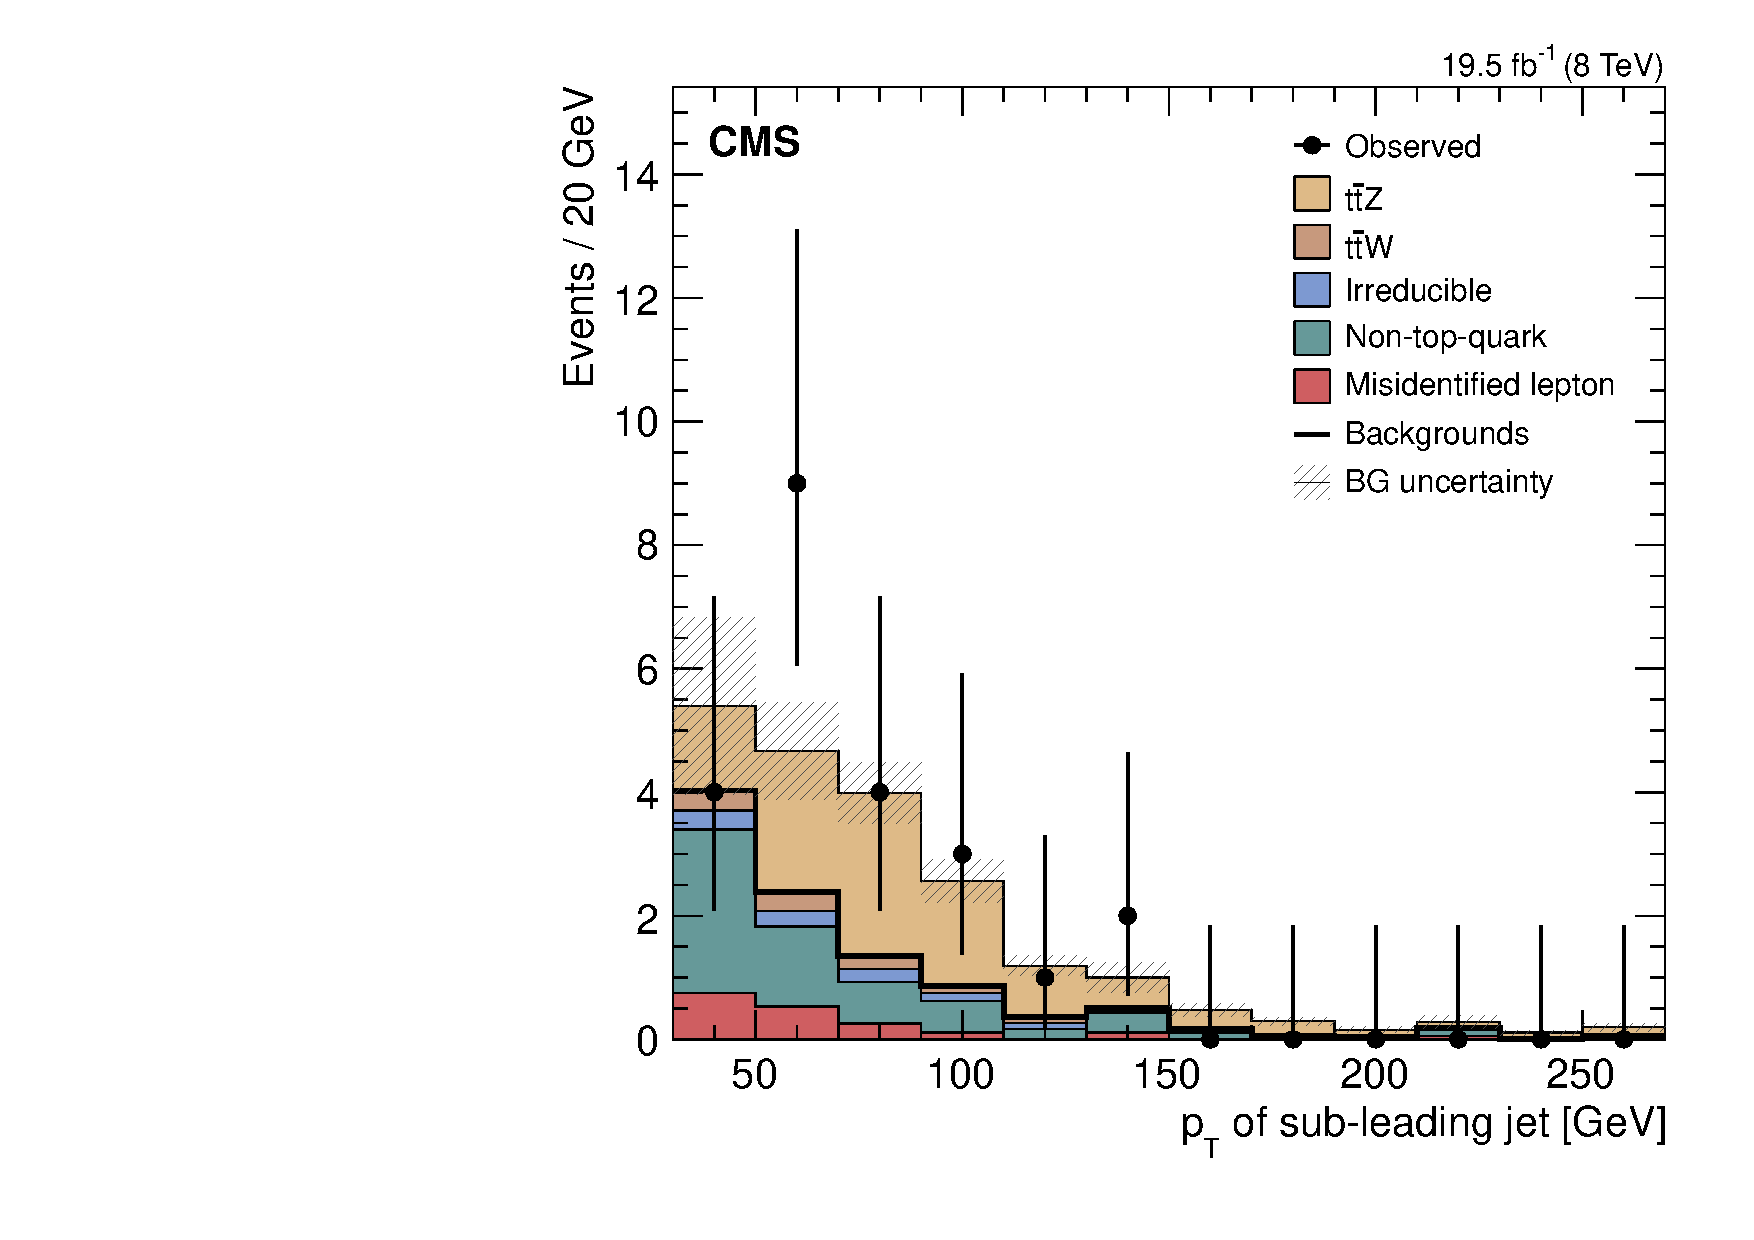
\includegraphics[width=0.48\linewidth]{Figs/Plots_PreSelections/hJ2Pt_3L2b.pdf}
\caption{\label{fig:JPt_3L2b}
Jet \pt . Left: \pt of leading jet after tri-lepton plus two b-tag selections. Right: \pt of sub leading jet after tri-lepton plus two b-tag selections.
}
\end{center}
\end{figure}


\begin{figure}[h]
\begin{center}
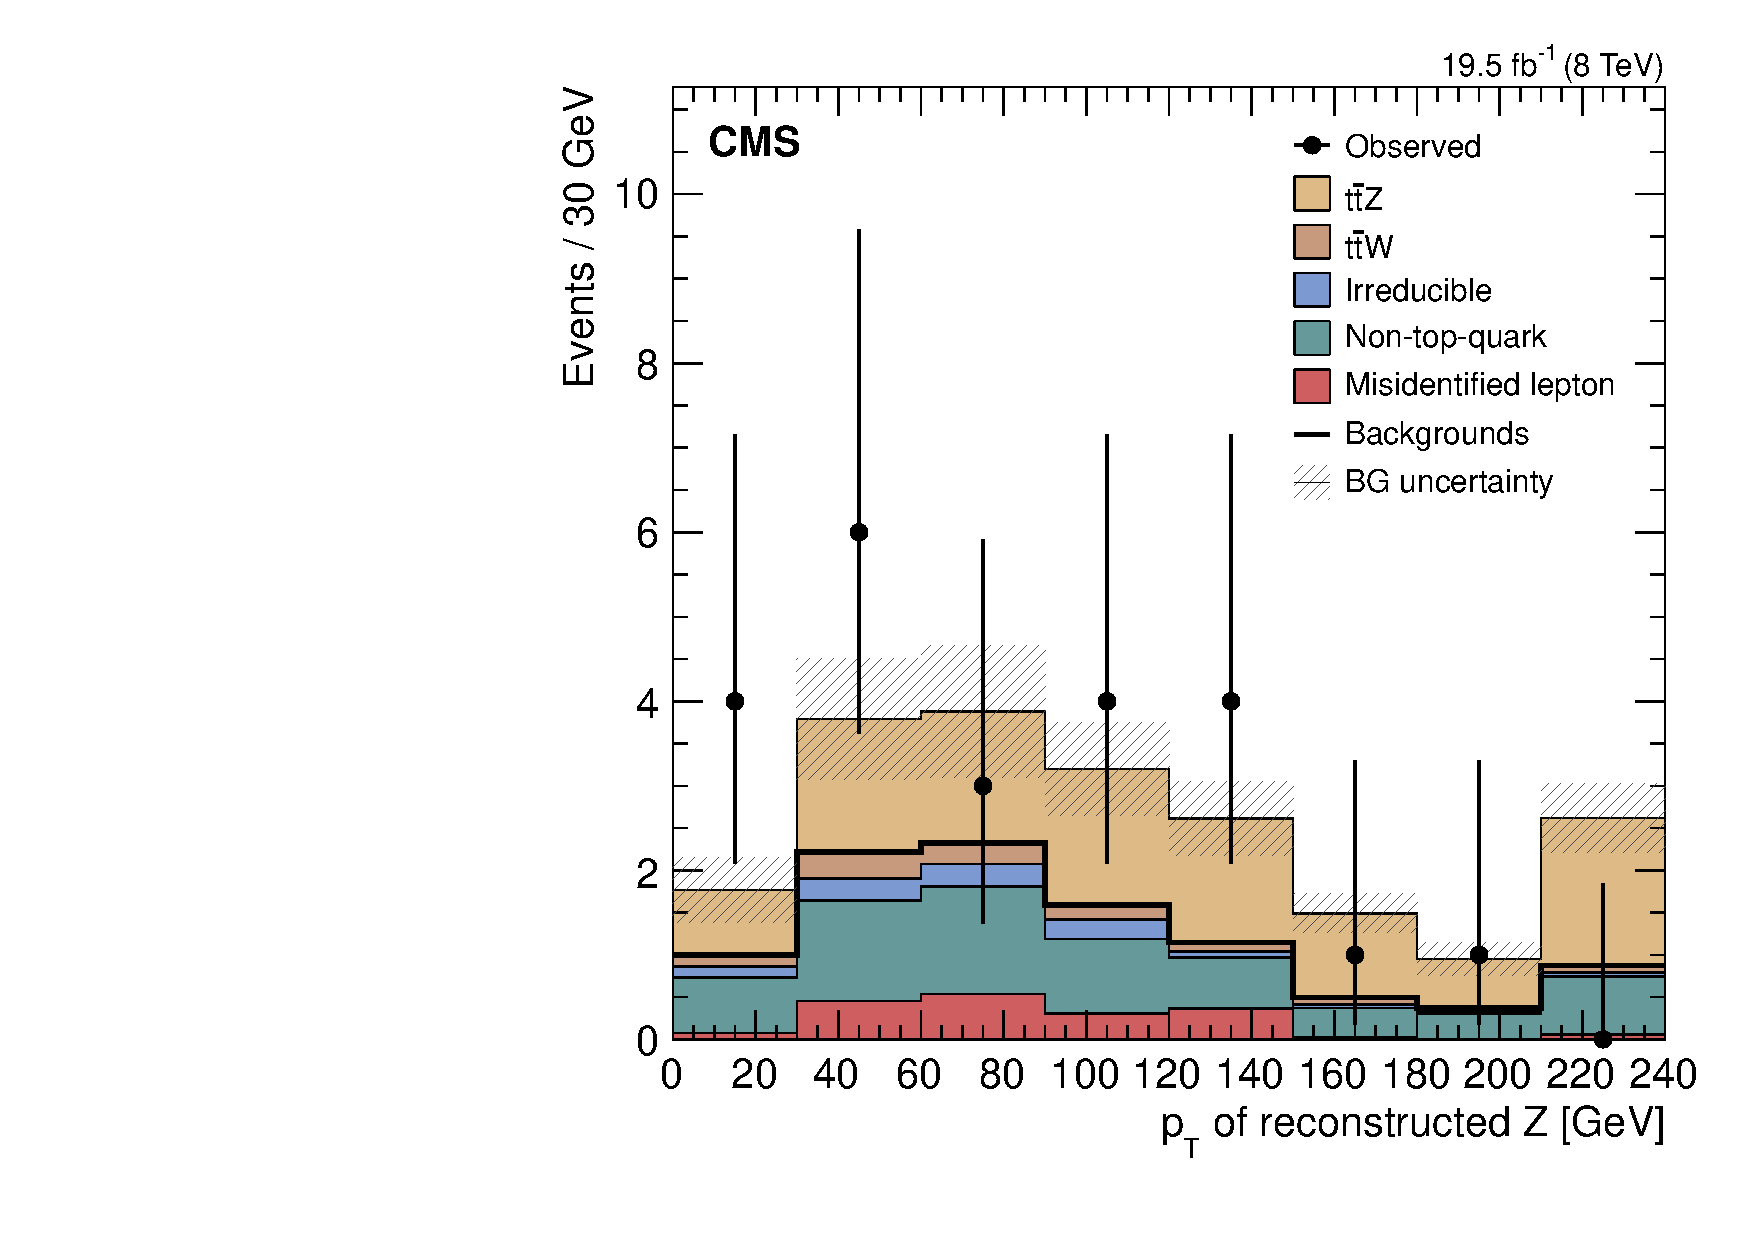
\includegraphics[width=0.48\linewidth]{Figs/Plots_PreSelections/hZPt_3L2b.pdf}
%\includegraphics[width=0.48\linewidth]{place_holders/index.png}
\caption{\label{fig:hzpt_3L2b}
\pt of the reconstructed Z boson after tri-lepton plus two b-tag selections.
}
\end{center}
\end{figure}

\clearpage

%\section{\ttZ Selection}
%The following figures contain additional plots of kinematic variables for the finals selection.
%
%\begin{figure}[h]
%\begin{center}
%\includegraphics[width=0.48\linewidth]{Figs/Plots_Final_Selections/hZLep1Pt_3L2J2b.pdf}
%\includegraphics[width=0.48\linewidth]{Figs/Plots_Final_Selections/hZLep2Pt_3L2J2b.pdf}
%\includegraphics[width=0.48\linewidth]{Figs/Plots_Final_Selections/hWLepPt_3L2J2b.pdf}
%\caption{\label{fig:hleppt_3L2J2b}
%\pt of the Z and W leptons after tri-lepton plus four jets (two of which are b-tag) selections . Left: Leading Pt lepton. Right: Trailing \pt lepton. Bottom: W lepton.
%}
%\end{center}
%\end{figure}
%
%
%
%
%\begin{figure}[h]
%\begin{center}
%\includegraphics[width=0.48\linewidth]{Figs/Plots_Final_Selections/hJ1Pt_3L2J2b.pdf}
%\includegraphics[width=0.48\linewidth]{Figs/Plots_Final_Selections/hJ2Pt_3L2J2b.pdf}
%\caption{\label{fig:JPt_3L2J2b}
%Jet \pt . Left: \pt of leading jet after tri-lepton plus four jets (two of which are b-tag) selections. Right: \pt of sub leading jet after tri-lepton plus two b-tag selections.
%}
%\end{center}
%\end{figure}
%
%
%\begin{figure}[h]
%\begin{center}
%\includegraphics[width=0.48\linewidth]{Figs/Plots_Final_Selections/hZPt_3L2J2b.pdf}
%%\includegraphics[width=0.48\linewidth]{place_holders/index.png}
%\caption{\label{fig:hzpt_3L2J2b}
%\pt of the reconstructed Z boson after tri-lepton plus four jets (two of which are b-tag) selections.
%}
%\end{center}
%\end{figure}
%
